\section{Jistá výhra}

\begin{enumerate}
    \item Jaká je optimální sázka maximalizující jistou výhru a jaká je její hodnota?

    Hodnoty sázek pro jednotlivé události:
    \[ \lr{x_1, x_2, x_3, x_4, x_5} = \lr{0, 2694.6, 0, 0, 305.4} \]
    Minimální hodnota výhry je \( \lambda = 2748.5 \).

    \item Pro modifikovanou slovní úlohu formulujte LP, která opět nalezne strategii sázení maximalizující minimální výhru.

    \[ \lr{\bf{x}^*, \lambda^*} \in \argmin_{\substack{\bf{x} \in \bbR^5 \\ \lambda \in \bbR}} - \lambda \]

    za podmínky
    \[
    \begin{array}{rcl}
        1.27 x_1 & \geq & \lambda \\
        4.70 x_2 & \geq & \lambda \\
        9 x_3 & \geq & \lambda \\
        \displaystyle \sum_{i = 1}^3 x_i & = & 3000 \\
        x_i & \geq & 400, \quad i = \left\{ 1, 2, 3 \right\}
    \end{array}
    \]

    Pro takto zadaný LP máme hodnotu jednotlivých sázek pro jednotlivé události
    \[ \lr{x_1, x_2, x_3} = \lr{2046.9, 553.1, 400} \]
    a hodnota minimální výhry je \( \lambda = 2599.6 \).
    
\end{enumerate}

\section{Minimaxní prokládání lineární funkce množinou bodů}

\begin{enumerate}
    \item Nalezenou optimální přímku vykreslete do grafu. Jaká je maximální absolutní odchylka pro tuto přímku?

    \begin{figure}[H]
        \centering
        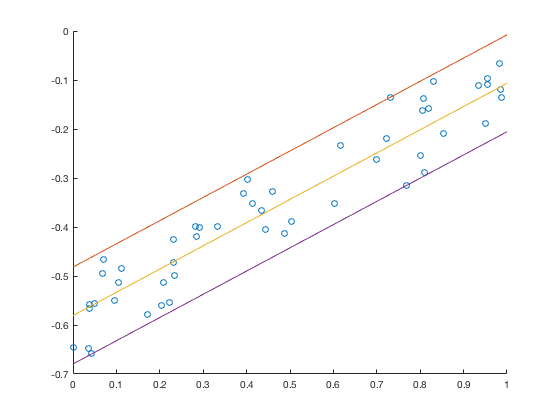
\includegraphics[width=0.8\textwidth]{../lp-primky.png}
        \caption{Graf optimalní přímky (žlutě) prokládající body v rovině}
    \end{figure}

    Maximální odchylka od přímky je \( \lambda = 0.0988 \).

    \item Přeformulujte úlohu pro případ, kdy \( x_i, i = 1, \dots, m \), jsou vektory z \( \bbR^n \). Vyjádřete tuto úlohu jako problém LP.

    \[ \lr{\bf{a}^*, b^*} \in \argmin_{\substack{\bf{a} \in \bbR^n \\ b \in \bbR \\ \lambda \in \bbR}} \lambda \]

    za podmínky
    \[
    \begin{array}{rcl}
        a_i x_{i,1} + \cdots + a_i x_{i, n} + b - y_i & \leq \lambda, \quad i = \left\{ 1, \dots, m \right\} \\
        -a_i x_{i,1} - \cdots - a_i x_{i, n} - b + y_i & \leq \lambda, \quad i = \left\{ 1, \dots, m \right\}
    \end{array}
    \]


\end{enumerate}